\documentclass[12pt,a4paper]{article}
\usepackage{amsfonts, amssymb, amsmath}
\usepackage{fullpage}
\usepackage{parskip} % skip a line instead of indenting
% \usepackage{graphicx} % for inserting images
\usepackage{amsthm}
\usepackage{xcolor}
\usepackage{tikz} % for plot

\title{Proves}
\author{R4 Cheng}
\date{\today}

\newcommand{\remark}[1]{
    $>$ {\color{blue} #1}
}

\begin{document}
\maketitle

\section*{Math}

\subsection*{Quadratic Form}

$\nabla \vec{x}^T\mathbf{A}\vec{x} = \vec{x}^T(\mathbf{A} + \mathbf{A}^T)$

if $\mathbf{A}$ is symmetric, then $\nabla_{\vec{x}} \vec{x}^T\mathbf{A}\vec{x} = 2\vec{x}^T\mathbf{A}$

Why is this important?

Almost all smooth nonlinear functions can be approximated by a quadratic function near a local minimum or maximum.

\subsection*{Inverse Matrix}

\[[ A \mid I ] \xrightarrow{} [ I \mid A^{-1} ]\]

E.g. $A = \begin{bmatrix} 1 & 2 \\ 3 & 4 \end{bmatrix}$

\[\left[ \begin{array}{cc|cc} 1 & 2 & 1 & 0 \\ 3 & 4 & 0 & 1 \end{array} \right]\]
\[\Rightarrow \left[ \begin{array}{cc|cc} 1 & 0 & -2 & 1 \\ 0 & 1 & 1.5 & -0.5 \end{array} \right]\]
\[\Rightarrow A^{-1} = \begin{bmatrix} -2 & 1 \\ 1.5 & -0.5 \end{bmatrix}\]


\subsection*{Symmetric Matrix}

\[\mathbf{A} = \mathbf{A}^T\]

\subsection*{Hessian Matrix}

\begin{itemize}
    \item It is a symmetric matrix.
\end{itemize}

\[
H = 
\nabla^2 f(\vec{x}) = 
\begin{bmatrix}
    \frac{\partial^2 f}{\partial x^2} & \frac{\partial^2 f}{\partial x \partial y} \\
    \frac{\partial^2 f}{\partial y \partial x} & \frac{\partial^2 f}{\partial y^2}
\end{bmatrix} = 
\begin{bmatrix} f_{xx} & f_{xy} \\ f_{yx} & f_{yy} \end{bmatrix}
\]

\remark{For continuous functions, $f_{xy} = f_{yx}$, so Hessian matrix is symmetric.}

Determinant of Hessian:

\[
H = \begin{bmatrix} A & B \\ B & C \end{bmatrix}
\Rightarrow \det(H) = AC - B^2
\]

\subsubsection*{Find Eigenvalues of Hessian}

Build characteristic equation:

\[\det(H - \lambda I) = 0\]
\[\Rightarrow
\det
\begin{bmatrix}
    f_{xx} - \lambda & f_{xy} \\
    f_{yx} & f_{yy} - \lambda
\end{bmatrix} = 0
\]
\[\Rightarrow (f_{xx} - \lambda)(f_{yy} - \lambda) - (f_{xy})(f_{yx}) = 0 \text{, } (a\lambda^2 + b\lambda + c = 0)\]

The roots $\lambda_1$ and $\lambda_2$ are the eigenvalues of $H$.

For each critial point $x_0$:

\begin{itemize}
    \item If both eigenvalues are positive, then $x_0$ is a local minimum.
    \item If both eigenvalues are negative, then $x_0$ is a local maximum.
    \item If eigenvalues have different signs, then $x_0$ is a saddle point.
    \item If any eigenvalue is zero, the test is inconclusive.
\end{itemize}

\subsection*{Jacobian Matrix}

\[J = \frac{\partial \sigma(\mathbf{x})}{\partial \mathbf{x}} =
\begin{bmatrix}
\frac{\partial \sigma(x_1)}{\partial x_1} & \cdots & \frac{\partial \sigma(x_1)}{\partial x_n} \\
\vdots & \ddots & \vdots \\
\frac{\partial \sigma(x_n)}{\partial x_1} & \cdots & \frac{\partial \sigma(x_n)}{\partial x_n}
\end{bmatrix}\]

Since Sigmoid function is element-wise, the output $\sigma(x_i)$ only depends on input $x_i$ (other inputs are irrelevant).
Therefore, all non-diagonal entries of the Jacobian matrix are zero.

\[\Rightarrow J = \text{diag}\Big( \sigma(\mathbf{x}) \odot (\mathbf{1} - \sigma(\mathbf{x})) \Big)\]

\[\text{(Streamline) } \sigma'(\vec{x}) = \sigma(\vec{x}) \odot (\vec{1} - \sigma(\vec{x}))\]

\remark{A small linear algebra trick: multiplying a row vector by a diagonal matrix is equivalent to performing element-wise multiplication (the Hadamard product) between the two vectors}

\section*{Loss (Cost) function}

\remark{aka. how to reward a machine}

$L_2$:

\[J(\vec{w}) = \frac{1}{2} \sum_{(\vec{x}, y) \in D} (f_{\vec{w}}(\vec{x}) - y)^2 + \lambda\lVert\vec{w}\rVert_2^2\]

\remark{Euclidean norm: $\lVert\vec{w}\rVert_2 = \sqrt{w_0^2+w_1^2 + \dots + w_n^2}$}

$L_1$:

\[J(\vec{w}) = \frac{1}{2} \sum_{(\vec{x}, y) \in D} (f_{\vec{w}}(\vec{x}) - y)^2 + \lambda\lVert\vec{w}\rVert_1^2\]

\remark{Manhattan norm: $\lVert\vec{w}\rVert_1 = |w_0| + |w_1| + \dots + |w_n|$}


Target:

\[\min_{\vec{w}} J(\vec{w})\]

\subsection*{Loss functions for classification}

\[\min_{\theta} \mathbb{E}_{x,y} [ \mathbb{I}[yf(x;\theta) \le 0] ]\]

If we are relying on gradients; why we pick a loss function that is upper bound of the 0-1 loss?

\[L_{Proxy}(x) \ge L_{0/1}(x)\]

A: As long as you can drive the upper bound very low, your true error rate will definitely also be low.

Options:

\begin{itemize}
    \item L1: $L_1 = |yf(x; \theta) - 1|$
    \item L2: $L_2 = (yf(x; \theta) - 1)^2$
    \item Hinge: $L_{\text{Hinge}} = \max(0, 1 - yf(x; \theta))$
    \item Cross Entropy: $L_{\text{CE}} = \log_2(1 + e^{-yf(x; \theta)})$
\end{itemize}

\subsection*{Loss functions for Regression}

\begin{itemize}
    \item L2 Loss (Squared Error / MSE): $L_2(y, f(x)) = (y - f(x))^2$
    \item L1 Loss (Absolute Error / MAE): $L_1(y, f(x)) = |y - f(x)|$
    \item Huber Loss: 
    \[L_{\delta}(y, f(x)) = \begin{cases}
    \frac{1}{2}(y - f(x))^2 & \text{for } |y - f(x)| \le \delta\\
    \delta(|y - f(x)| - \frac{1}{2}\delta) & \text{otherwise}
    \end{cases}\]
\end{itemize}

\section*{Gradient Descent}

\subsection*{(Batch) Gradient Descent}

\[\min f(a + \Delta x) \approx \min f(a) + \nabla f(a)^T \Delta x\]
\[\Rightarrow \nabla f(a)^T \Delta x\text{ should be as minus as possible}\]

\[v^T w = \|v\| \|w\| \cos \theta\]
\[\Rightarrow \nabla f(a)^T \Delta x = \|\nabla f(a)\| \|\Delta x\| \cos \theta\]
\[\text{To max minus } \Rightarrow \cos \theta = -1 \Rightarrow \theta = 180^\circ\]
\[\Rightarrow \Delta x = - \alpha \nabla f(a)\]
$\Rightarrow$

We control the step size with $\alpha$ (learning rate) to minimize $f(a - \alpha \nabla f(a))$.

\rule{\linewidth}{0.4pt}

(Another way) Start from an arbitrary initial weight vector $\vec{w}$.

\[\vec{w'} \leftarrow \vec{w} - \alpha \Delta J(\vec{w}) = \vec{w} - \alpha \frac{\partial}{\partial \vec{w}}J(\vec{w})\]

\remark{$\alpha$ is called learning rate}

And for a single training example $(\vec{x}, y)$, we have:

\[\vec{w'} \leftarrow \vec{w} - \alpha(\vec{w} \cdot \vec{x} - y)\vec{x} = \vec{w} + \alpha(y - \vec{w} \cdot \vec{x})\vec{x}\]

Aka. the least mean square (LMS) udpate rule.

\remark{vs perceptron: $\vec{w'} = \vec{w} + y\cdot\vec{x}$}

\begin{align*}
Derivation:
\frac{\partial}{\partial \vec{w}}J(\vec{w}) &= \frac{\partial}{\partial \vec{w}}\frac{1}{2}(f(\vec{x}) -y)^2\\
&= 2 \cdot \frac{1}{2}(f(\vec{x}) - y) \cdot \frac{\partial}{\partial \vec{w}}(f(\vec{x}) - y) \quad \text{// Chain Rule}\\
&= (\vec{w} \cdot \vec{x} - y) \cdot \frac{\partial}{\partial \vec{w}}(\vec{w} \cdot \vec{x} - y)\\
&= (\vec{w} \cdot \vec{x} - y)\vec{x}
\end{align*}

Therefore, for the whole dataset $D$:

\[\vec{w'} \leftarrow \vec{w} + \alpha \sum_{(\vec{x},y) \in D}(y - \vec{w} \cdot \vec{x}) \vec{x}\]

\subsection*{Stochastic Gradient Descent}

Streamline BGD:

\[\vec{w'} \leftarrow \vec{w} + \alpha(y_i - \vec{w} \cdot \vec{x}_i)\vec{x}_i\]

Where $(\vec{x}_i, y_i)$ is a randomly picked training example from $D$.

\subsection*{Mini-Batch Gradient Descent}

\remark{Balance between GD and SGD}

\[\vec{w'} \leftarrow \vec{w} + \alpha \sum_{(\vec{x},y) \in D_m}(y - \vec{w} \cdot \vec{x})\vec{x}\]

Where $D_m \subset D$ is a randomly picked $m$ examples of training data.

\subsection*{Stochastic Gradient Descent with Momentum}

\[m^{(t+1)} = \mu m^{(t)} - \alpha \nabla L(\theta^{(t)})\]
\[\theta^{(t+1)} = \theta^{(t)} + m^{(t+1)}\]

\remark{E.g. if $\mu$ is 0.9, it means we keep 90\% old velocity.}

\remark{Typically set $\mu$ to 0.8 - 0.9 (rule-of-thumb)}

\subsection*{Ridge regression gradient descent}

\remark{$L_2$, becuase it is differentiable}

\[\vec{w'} \leftarrow \vec{w} + \alpha \sum_{(\vec{x},y) \in D}(y - \vec{w} \cdot \vec{x}) \vec{x} - \lambda \vec{w}\]

The function of $\lambda \vec{w}$ is to decrease the magnitude of $\vec{w}$, leading to reduced model complexity and overfitting.

\section*{Normal Equation}

TODO

\section*{Deep Learning}

\subsection*{Activation Functions}

The activation function introduces non-linearity into the model (network), enabling it to learn and represent complex patterns in the data.

\remark{elementwise}

\begin{itemize}
    \item Sign: $\text{sign}(x) = \begin{cases}
    1 & \text{if } x \ge 0\\
    -1 & \text{if } x < 0
    \end{cases} \Rightarrow$ Simple binary output. (Not differentiable, not good for backpropagation)
    \item Sigmoid: $\sigma(x) = \frac{1}{1 + e^{-x}} \Rightarrow$ Usually for binary classification questions.
    
    \begin{center}
    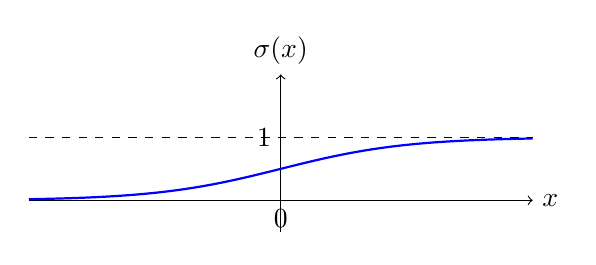
\begin{tikzpicture}[scale=0.8]
        \draw[->] (-4,0) -- (4,0) node[right] {$x$};
        \draw[->] (0,-0.5) -- (0,2) node[above] {$\sigma(x)$};
        \draw[blue, thick, domain=-4:4, samples=100] plot (\x, {1/(1+exp(-\x))});
        \draw[dashed] (-4,1) -- (4,1);
        \node[below] at (0,0) {$0$};
        \node[left] at (0,1) {$1$};
    \end{tikzpicture}
    \end{center}
    
    \item Hyperbolic Tangent (Tanh): $\tanh(x) = \frac{e^x - e^{-x}}{e^x + e^{-x}} \Rightarrow$ Make data zero-centered which can speed up convergence.
    
    \begin{center}
    \begin{tikzpicture}[scale=0.8]
        \draw[->] (-4,0) -- (4,0) node[right] {$x$};
        \draw[->] (0,-2) -- (0,2) node[above] {$\tanh(x)$};
        \draw[blue, thick, domain=-4:4, samples=100] plot (\x, {tanh(\x)});
        \draw[dashed] (-4,1) -- (4,1);
        \draw[dashed] (-4,-1) -- (4,-1);
        \node[below] at (0,0) {$0$};
        \node[left] at (0,1) {$1$};
        \node[left] at (0,-1) {$-1$};
    \end{tikzpicture}
    \end{center}
    
    \item Rectified Linear Unit (ReLU): $\text{ReLU}(x) = \max(0, x) \Rightarrow$ Only allows positive values to pass through.
    
    \begin{center}
    \begin{tikzpicture}[scale=0.8]
        \draw[->] (-4,0) -- (4,0) node[right] {$x$};
        \draw[->] (0,-0.5) -- (0,3) node[above] {$\text{ReLU}(x)$};
        \draw[blue, thick] (-4,0) -- (0,0);
        \draw[blue, thick] (0,0) -- (3,3);
        \node[below] at (0,0) {$0$};
    \end{tikzpicture}
    \end{center}

    \remark{It makes training deep neural networks much easier.}

    \item Leaky ReLU: $\text{Leaky ReLU}(x) = \begin{cases}
    x & \text{if } x > 0\\
    \alpha x & \text{if } x \le 0
    \end{cases} \Rightarrow$ Prevents dying ReLU problem.

    $\text{Leaky ReLU}'(x) = \begin{cases}
    1 & \text{if } x > 0\\
    \alpha & \text{if } x \le 0
    \end{cases}$

    \item Softmax: $\text{Softmax}(z_i) = \frac{e^{z_i}}{\sum_{j} e^{z_j}} \Rightarrow$ Converts logits into probabilities for multi-class classification. (the only non-elementwise)
\end{itemize}

\subsection*{Backpropagation}

An algorithm way to efficiently compute parameter gradients. $\Rightarrow$ Its work is only until getting $\nabla_\theta Loss$

\remark{Optimizer will use the list generated by backpropagation to update parameters.}

For the l-th layer, with weights $W^{(l)}$, the gradient for that layer is:

\[\nabla_{W^{(l)}} L = \boldsymbol{\delta}^{(l)} (\mathbf{a}^{(l-1)})^T\]

\[\mathbf{a}^{(l-1)} \xrightarrow[\text{weights computation}]{W^{(l)}} \mathbf{z}^{(l)}
\xrightarrow[\text{activation function}]{\sigma(\cdot)} \mathbf{a}^{(l)}\]

\remark{$\boldsymbol{\delta}^{(l)} = \frac{\partial L}{\partial \mathbf{z}^{(l)}} = \frac{\partial a^{(l)}}{\partial z^{(l)}}\frac{\partial L}{\partial a^{(l)}} = \sigma'(z^{(l)})\frac{\partial L}{\partial a^{(l)}}$}

\subsection*{Why and When to use CNN?}

\begin{itemize}
    \item A neuron does not have to see the whole image to discover the pattern.
    \item The same patterns appear in different locations of the image. $\Rightarrow$ two neurons in different locations can share the same weights.
    \item Subsampling (pooling) can reduce the dimensionality of the image while preserving important features.
\end{itemize}

N filters is equivalent to one fully connected layer with a neuron.

The parameters in the filter should be learned like normal weights and biases in NN.

\subsection*{Weight Decay}

\remark{Actually, it is almost the synonym of L2 Regularization; it is just from the perspective of update rule.}

\[\theta^{(t+1)} = \theta^{(t)} - \alpha \nabla L(\theta^{(t)}) \mathbf{- 2\alpha\lambda\theta}\]

\subsection*{Word Embeddings}

\subsubsection*{Cosine Similarity}

Cosine similarity measures the relationship between word vectors in an embedding space.

\[\text{Cosine Similarity}(\mathbf{A}, \mathbf{B}) = \frac{\mathbf{A} \cdot \mathbf{B}}{\|\mathbf{A}\| \|\mathbf{B}\|} = \frac{\sum_{i=1}^{n} A_i B_i}{\sqrt{\sum_{i=1}^{n} A_i^2} \sqrt{\sum_{i=1}^{n} B_i^2}}\]
\[-1 \ge \text{Cosine Similarity}(\mathbf{A}, \mathbf{B}) \le 1\]

\begin{itemize}
    \item $1$: Vectors are identical (high semantic similarity)
    \item $0$: Vectors are orthogonal (no semantic similarity)
    \item $-1$: ?????
\end{itemize}

\subsubsection*{Dimensionality Reduction}

E.g. 7D to 2D

\remark{Using e.g. PCA, t-SNE, UMAP}

\subsubsection*{The objective function of the Skip-gram Model}

\section*{AlphaGo Zero}

\subsection*{The Deep Neural Network $f_{\theta}$}

\[(\vec{p},\,v) = f_{\theta}(s)\]

\begin{itemize}
    \item $s$: Input, the position and history of the game.
    \item $\vec{p}$: Output, the probability of selecting each move a (including pass), $p_a = Pr(a \mid s)$.
    \item $v$: Output, scalar evaluation, estimating the probability of the current player winning from position $s$.
\end{itemize}

\subsection*{MCTS search}

In each position $s$, an MCTS search is executed, guided by the neural network $f_{\theta}$.

Output $\pi$: probabilities of playing each move, usually better than $\vec{p} \Rightarrow$ powerful policy improvement operator.

\subsection*{The idea}

Update $\theta$ to let $(\vec{p}, v)$ be closer to $(\pi, z)$.

\remark{$z$: the game winner z}

\subsection*{Loss function}

\[l = (z - v)^2 - \pi^T \log \vec{p} + c\lVert\theta\rVert^2\]

The neural network parameters $\theta$ are updated to \textbf{maximize} the similarity of the policy vector $\vec{p}$ to the search probabilities $\pi_t$, 
and to \textbf{minimize} the error between the predicted winner $v_t$ and the game winner $z$.

\end{document}
